\documentclass[12pt,t,xcolor=dvipsnames]{beamer}
\usepackage{amsmath,amssymb}
\usepackage{multirow}
\usepackage{subfigure}
\usepackage{pgfplots}

\graphicspath{{figs/}}

% AMGr macros
\newcommand{\A}{A}%{\mathbb{A}}
\newcommand{\Mff}{M_{ff}}
\newcommand{\Mffinv}{M_{ff}^{-1}}
\newcommand{\Aff}{A_{ff}}
\newcommand{\Affinv}{A_{ff}^{-1}}
\newcommand{\Aschur}{\hat{A}_{cc}}
\newcommand{\Aschurinv}{\hat{A}_{cc}^{-1}}
\newcommand{\Afc}{A_{fc}}
\newcommand{\Acf}{A_{cf}}
\newcommand{\Acc}{A_{cc}}
\newcommand{\half}{\frac{1}{2}}
\DeclareMathOperator*{\argmin}{argmin}
\renewcommand{\H}[1]{{#1}^\star}
\renewcommand{\vec}[1]{{\bf #1}}

% Beamer Commands
\setbeamertemplate{navigation symbols}{}
\setbeamertemplate{footline}
{%
\hspace*{0.7\linewidth}\insertshorttitle - p.\insertframenumber
}
\setbeamertemplate{footnote}
{%
\insertfootnotetext
}
\setbeamercolor{footnote mark}{fg=white}
\setbeamertemplate{frametitle}[default][center]
\setbeamertemplate{itemize item}[circle]
\setbeamertemplate{itemize subitem}[triangle]
\setbeamercolor{itemize subitem}{fg=Plum}
\setbeamerfont{itemize subitem}{size=\normalsize}
\setbeamercolor{alerted text}{fg=Magenta}
\setbeamerfont{institute}{size=\normalsize}
\setbeamerfont{list label}{series=\bfseries}
\usefonttheme[onlylarge]{structurebold} 

\newcommand{\alerta}[1]{{\usebeamercolor[fg]{frametitle} #1}}

% Title Page Stuff
\title{Multigrid Methods for Regularized Problems}
\author{Scott MacLachlan \\ Memorial University of Newfoundland \\ \texttt{smaclachlan@mun.ca}}
\date{March 28, 2017}
\institute{and \\ Matthias Bolten, Universit\"at Kassel \\ Misha Kilmer, Tufts University}

\renewcommand{\vec}[1]{{\bf #1}}


\begin{document}

% Title Page
% - Begin Slide -----
\maketitle

% Application
% - Begin Slide -----
\begin{frame}
  \frametitle{Motivation: Inverse Problems}

  Consider Radon Transform:\\ Let $f(x,y)$ be unknown density in a
  region, $\Omega \subset \mathbb{R}^2$.  Given line, $L$, whose
  minimum distance to the origin is $s$ and whose normal vector makes
  angle $\alpha$ to $x$-axis, compute
  \[
(Rf)(s,\alpha) = \int_{-\infty}^{\infty} f(z\sin\alpha+s\cos\alpha,-z\cos\alpha+s\sin\alpha)dz
  \]

  \begin{minipage}{0.48\textwidth}
  \alert{Inverse Problem:} Given set of computed values
  $(Rf)(s,\alpha)$, can we reconstruct $f(x,y)$ pixelwise to match
  data?
  \end{minipage}
  \begin{minipage}{0.48\textwidth}
    \begin{center}
      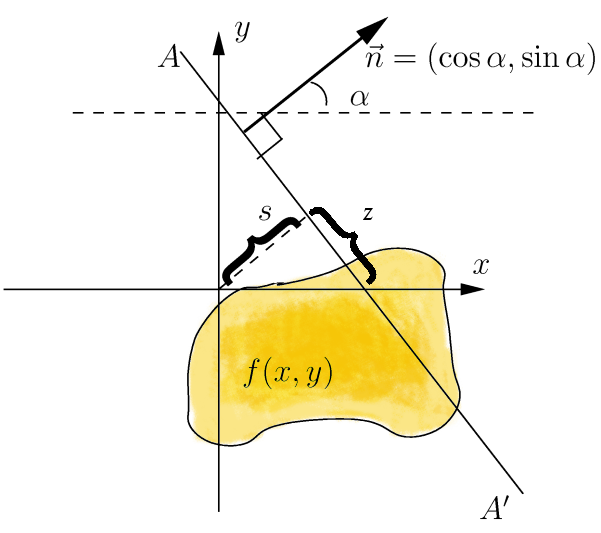
\includegraphics[width=0.7\linewidth]{Radon_transform} \\
      {\tiny From wikipedia, attribution: Begemotv2718 from ru}
    \end{center}
  \end{minipage}
  

\end{frame}

% - Begin Slide -----
\begin{frame}
  \frametitle{Ill-Posed Problem\footnote{PC Hansen, {\it Discrete
        Inverse Problems:\ Insight and Algorithms}, SIAM 2010}}

  Let $K$ be the matrix that encodes Radon Transform, $\vec{b}^{\text{true}}$ be
  ``clean'' data generated, and $\vec{b} =
  \vec{b}^{\text{true}}+\vec{e}$ be noisy data. \\[12pt]

  \alert{Na\"ive approach:} Solve $K\vec{x} = \vec{b}$.\\[12pt]

  \pause
  Issues:
  \begin{itemize}
  \item $K$ may not be square
    \begin{itemize}
    \item Number of measurements need not match number of pixels
      \item Try least-squares solution? $K^TK\vec{x} = K^T\vec{b}$
    \end{itemize}
    \pause

  \item $K$ has poor spectral structure
    \begin{itemize}
    \item Singular values decay to zero
    \item Small singular values associated with high-frequency modes
    \item Noise is amplified in least-squares solution
    \end{itemize}
    
    
  \end{itemize}
  

\end{frame}

% - Begin Slide -----
\begin{frame}
\frametitle{Regularization\footnote{PC Hansen, {\it Discrete
        Inverse Problems:\ Insight and Algorithms}, SIAM 2010}}
Overcome ill-posedness of inverse problem by adding term
\[
K\vec{x} = \vec{b} \quad \Rightarrow \quad \min_{\vec{x}}
\|K\vec{x}-\vec{b}\|_2^2 + \lambda^2\|L\vec{x}\|_2^2
\]

Notes:
\begin{itemize}
\item Use parameter $\lambda$ to balance between data fidelity and
  regularization term
\item ``Classic'' choices in many settings are $L=I$ or $L = $
  discrete gradient
\begin{itemize}
\item Neither suitable for many imaging applications
\end{itemize}
\end{itemize}

\end{frame}

% - Begin Slide -----
\begin{frame}
\frametitle{Changing Norms}
Expect solutions to inverse problem to be piecewise constant functions
\begin{itemize}
\item Physical structures composed of distinct materials
\item For discrete gradient, $L\vec{x}$ is zero in regions where $\vec{x}$ is constant, but
  has large jumps on boundaries
  \begin{itemize}
  \item Euclidean norm strongly penalizes these jumps, leading to too
    much smoothing
    \item Other norms do better: $\ell^1$, TV
  \end{itemize}
  
\end{itemize}
\ \\[12pt]

\pause
\alert{Goal:} Solve $\displaystyle\min_{\vec{x}}
\|K\vec{x}-\vec{b}\|_2^2 + \lambda^2\|L\vec{x}\|_\ast^2$
\begin{itemize}
\item Non-quadratic form, so derivative is nonlinear
  \end{itemize}
\end{frame}

% - Begin Slide -----
\begin{frame}
  \frametitle{Linearization\footnote{O Semerci, {\it Image Formation
        Methods for Dual Energy and Multi-Energy Computed Tomography},
      PhD thesis 2012, Tufts University\\
  Kilmer, Semerci, Miller, {\it An Adaptive Inner-Outer Iterative
Regularization Method for Edge Recovery}, presented at ICIAM 2015}}
  Replace nonquadratic minimization with sequence of quadratic
  problems:\\[-24pt]
  \[
\min_{\vec{x}^{(i)}}
\|K\vec{x}^{(i)}-\vec{b}\|_2^2 + \lambda_i^2\|L^{(i)}\vec{x}^{(i)}\|_2^2
  \]

  \alert{Idea:} replace discrete gradient by weighted term that converges to
  $\ell^1$/TV-type norm. \\[6pt]

  Outer iteration: given $L^{(0)} = L$, $\Lambda^{(0)} = I$, $\vec{x}^{(0)}$
  \begin{itemize}
  \item Compute $\vec{v} = L^{(0)}\vec{x}^{(i-1)}$
  \item Normalize $\vec{v} \leftarrow \vec{v}/\|\vec{v}\|_\infty$
  \item Take $\vec{d} = 1-\vec{v}.^2$ (or $\vec{d} = 1-|\vec{v}|$)
  \item Define $\Lambda^{(i)} = \text{diag}(\vec{d})$, $L^{(i)} =
    \Lambda^{(i)}L^{(i-1)}$
    \item Take $\vec{x}^{(i)}$ to minimize $\|K\vec{x}^{(i)}-\vec{b}\|_2^2 + \lambda_i^2\|L^{(i)}\vec{x}^{(i)}\|_2^2$
  \end{itemize}
  
\end{frame}

% - Begin Slide -----
\begin{frame}
  \frametitle{Choosing $\lambda_i$}
  
  Choose $\lambda_i$ by solving for several values \& picking best \\[9pt]

Minimize $\|K\vec{x}^{(i,\ell)}-\vec{b}\|_2^2 + (\lambda^{(\ell)})^2\|L^{(i)}\vec{x}^{(i,\ell)}\|_2^2$
  for fixed set of values $\{\lambda^{(\ell)}\}$ \\[9pt]

  Choose $\lambda_i$ using L-curve, balancing relative size of two terms

  \begin{center}
      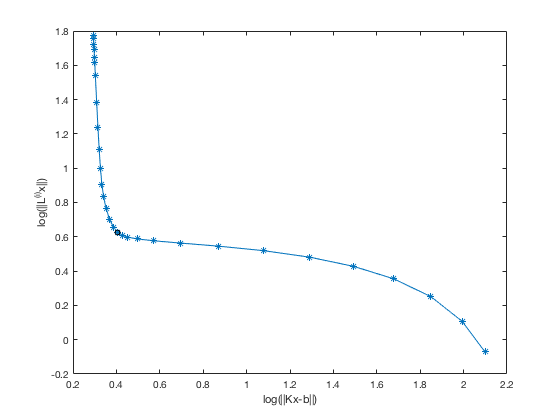
\includegraphics[width=0.65\linewidth]{Lcurve}
    \end{center}
  
\end{frame}

% - Begin Slide -----
\begin{frame}
  \frametitle{Lots of Linear Solves!}

  Have two nested loops
  \begin{itemize}
  \item Outer loop to linearize $\ell^1$/TV regularization term
  \item Middle loop to solve for each value of
      $\{\lambda^{(\ell)}\}$
    
  \end{itemize}

  For each $i$ and $\ell$, need to minimize
  \[
\|K\vec{x}^{(i,\ell)}-\vec{b}\|_2^2 + (\lambda^{(\ell)})^2\|L^{(i)}\vec{x}^{(i,\ell)}\|_2^2
\]

Now form normal equations:
\[
\left(K^TK + (\lambda^{(\ell)})^2(L^{(i)})^TL^{(i)}\right)\vec{x}^{(i,\ell)} = K^T\vec{b}
\]
\end{frame}

% - Begin Slide -----
\begin{frame}
  \frametitle{Connection to multigrid}

  Take $D^{(i)} =
  \left(\Lambda^{(i)}\Lambda^{(i-1)}\cdots\Lambda^{(0)}\right)^2$, so normal
  equations give
\[
\left(K^TK + (\lambda^{(\ell)})^2L^TD^{(i)}L\right)\vec{x}^{(i,\ell)} = K^T\vec{b}
\]

For ``large'' $\lambda^{(\ell)}$, system is dominated by $L^TD^{(i)}L$,
which is essentially an anisotropic diffusion operator \\[18pt]

\alert{Goal:} Leverage AMG to create a fast algorithm for normal equations

\end{frame}

% - Begin Slide -----
\begin{frame}
  \frametitle{Challenges}
  \begin{itemize}
  \item $K^TK$ is essentially dense
    \begin{itemize}
    \item For Radon transform $K\in\mathbb{R}^{6270\times4096}$,
      $K^TK$ is 80\% full
      \item Can't form matrix from normal equations
    \end{itemize}
  \item Want to reuse as much as possible
    \begin{itemize}
    \item $L^TD^{(i)}L$ only changes at outer iteration, form this
      once
    \item Only $\lambda^{(\ell)}$ changes in middle iteration
    \end{itemize}
  \item $\{\lambda^{(\ell)}\}$ spans several orders of magnitude
    \begin{itemize}
    \item No ``one size fits all'' solution
    \item Need to consider several distinct parameter ranges
    \end{itemize}
  \end{itemize}

\end{frame}

% - Begin Slide -----
\begin{frame}
\frametitle{Low-hanging fruit}

For largest values of $\lambda^{(\ell)}$, system is dominated by
$L^TD^{(i)}L$. \\[12pt]

Modify classical AMG:
\begin{itemize}
\item Compute strong connections and interpolation based only on
  $L^TD^{(i)}L$
\item Coarsen $K$ recursively in one-sided manner: $K_c = K_fP^f_c$
\item Iteration is V(1,0) cycle
\item Relaxation is weighted $CF$-Jacobi
  \begin{itemize}
  \item Aim to only use $K^T$ and $K$ via matvecs
  \item Gauss-Seidel is too expensive, due to density of $K^TK$
  \item Precompute diagonals of $K^TK$ and $L^TD^{(i)}L$
  \item Weighting depends on value of $\lambda^{(\ell)}$
  \end{itemize}
  
\end{itemize}

\end{frame}

% - Begin Slide -----
\begin{frame}
  \frametitle{Relative sizes}

  What does it mean for $\lambda^{(\ell)}$ to be ``large''? \\[12pt]

  Practical comparison:
  \begin{itemize}
  \item Estimate $\rho_K = \rho(K^TK)$ using Arnoldi
    \begin{itemize}
    \item Do this once for all iterations
    \end{itemize}
  \item Estimate $\rho_L = \rho(L^TD^{(i)}L)$ using Arnoldi
    \begin{itemize}
    \item Do this once per outer iteration
    \end{itemize}
  \end{itemize}
  \ \\[12pt] \pause

  Say that $\lambda^{(\ell)}$ is large when
  $(\lambda^{(\ell)})^2\rho_L > 100\rho_K$
  \begin{itemize}
  \item Potential to try and characterize using both ends of spectrum,
  but simpler criterion seems to work well
  \item Use
    $\left((\lambda^{(\ell)})^2\rho_L\right)/\left((\lambda^{(\ell)})^2\rho_L
    + \rho_K\right)$ as Jacobi relaxation weight
    \begin{itemize}
\item For largest $\lambda^{(\ell)}$, use no under-relaxation, since
  CF ordering is enough (approaches RBGS)
  \item Under-relaxation is important for lower range of
    $\lambda^{(\ell)}$ included in this case.
    \end{itemize}
    
  
  \end{itemize}
  

\end{frame}

% - Begin Slide -----
\begin{frame}
  \frametitle{Slightly higher fruit}

  For middle range of $\lambda^{(\ell)}$, AMG structure still
  effective, but weighted Jacobi is not \\[12pt]

  Alternate relaxation:
  \begin{itemize}
  \item Kaczmarz is too expensive
  \item SART/Cimmino (Jacobi-like on normal equations) are
    ineffective (parameter tuning?)
  \item Chebyshev on normal equations works, but requires parameter tuning
  \item PCGNE balances effectiveness and cost
    \begin{itemize}
    \item Use 3 steps of PCGNE for best(?) performance
      \item Diagonal scaling as preconditioner
    \end{itemize}
    
  \end{itemize}

\end{frame}

% - Begin Slide -----
\begin{frame}
\frametitle{High-hanging fruit}
Smallest $\lambda^{(\ell)}$ have opposite behaviour
\begin{itemize}
\item $K^TK$ is dominant operator, typical inverse problem structure
\item AMG based on $L^TD^{(i)}L$ is now a poor solver
\end{itemize}
\ \\[12pt]

Future work:
\begin{itemize}
\item For now, just use LSQR
\item Looking at symbol to see if we can use MG principles here
  
\end{itemize}


\end{frame}

% - Begin Slide -----
\begin{frame}
  \frametitle{Some details}

  Lots of potential for recycling to save costs
  \begin{itemize}
\item Start each outer iteration with optimal solution from previous one
  \item Within outer iterations, sweep through $\{\lambda^{(\ell)}\}$
    from largest to smallest
    \begin{itemize}
    \item Takes advantage of best performance for largest
      $\lambda^{(\ell)}$
    \item Generally see monotonic increase in optimal
      $\lambda^{(\ell)}$ as outer iterations proceed
    \item Potential to truncate this iteration once corner of
      L-curve is prominent
    \end{itemize}
    
  \end{itemize}
  
  Linear iteration stopping criterion:
  \begin{itemize}
  \item For now, reduction of $\ell^2$ norm of the residual of
  the normal equations below $10^{-4}$
  \begin{itemize}
  \item Absolute reduction since good quality initial guesses available
  \end{itemize}
  \end{itemize}
  
\end{frame}

% - Begin Slide -----
\begin{frame}
\frametitle{Test problem}

Standard Shepp-Logan phantom
\begin{itemize}
\item $64^2$ pixels in image
\item Limited angle: 130 degrees in 2 degree increments
\end{itemize}


  \begin{minipage}{0.48\textwidth}
    \begin{center}
      
\includegraphics[width=0.9\linewidth]{SheppLogan}
    \end{center}
  \end{minipage}
  \begin{minipage}{0.48\textwidth}
Consider 3 different noise\\ levels: 0.5\%, 1\%, 2\% \\ (Additive
Gaussian Noise)
  \end{minipage}

  For now, run 15 outer iterations
  \begin{itemize}
  \item Outer iteration stopping tolerance still an open question
    \begin{itemize}
      \item Simple form of weight update doesn't quite correspond to
      nonlinear minimization.
    \end{itemize}
  \end{itemize}
  
\end{frame}

% - Begin Slide -----
\begin{frame}
  \frametitle{Selection of $\lambda_i$}

  Consider $\{\lambda^{(\ell)}\}$ with 30 values logarithmically spaced between
  $0.001$ and $100$ \\[12pt]

  \hspace*{-1cm}
  \setlength\tabcolsep{1.5pt}
  \begin{tabular}{l|ccccc|ccccc|ccccc}
    Noise & 1 & 2 & 3 & 4 & 5 & 6 & 7 & 8 & 9 & 10 & 11 & 12 & 13 & 14
    & 15 \\
    \hline
    0.5\% & .016 &  .024 &  .036 &  .053 &  .079 &    .079 &    .12 &
    .12 &    .17 &    .26 &    .39 & .57 &    \alerta{1.3} &    \alerta{2.8} &    \alerta{6.2}\\
    1\% & .036 &   .036  &  .079 &   .12 &    .12 &    .17 &
    .26 &    .57 &    \alerta{.85} &    \alerta{1.3} &    \alerta{1.9} & \alerta{2.8} &   \alerta{4.2} &
    \alerta{4.2} &    \alerta{6.2}\\
    2\% & .053 &    .079 &   .12 &   .17 &    .57 &    \alerta{.85} &    \alerta{1.3} &
    \alerta{1.9} &    \alerta{2.8} &    \alerta{6.2} &    \alerta{6.2} & \alerta{13.7} &  \alerta{20.4} &   \alert{30.4} &   \alert{45.2}\\
   \end{tabular}

  \ \\[12pt]
  \begin{itemize}
  \item Steady increase in $\lambda_i$ selected with outer iteration
  \item General trend to large $\lambda_i$ with more noise
  \end{itemize}

\end{frame}


% - Begin Slide -----
\begin{frame}
\frametitle{Solutions generated}

\hspace*{-1cm}
  
\includegraphics[width=0.4\linewidth]{Solution_05}
  
\includegraphics[width=0.4\linewidth]{Solution_1}
  
\includegraphics[width=0.4\linewidth]{Solution_2}

0.5\% Noise \hfill 1\% Noise \hfill 2\% Noise

\ \\[12pt]
  Note strong effect of noise on error in solutions
  \begin{itemize}
    \item 0.5\% noise $\rightarrow$ 0.65\% relative error
    \item 1\% noise $\rightarrow$ 9.1\% relative error
    \item 2\% noise $\rightarrow$ 29.8\% relative error
  \end{itemize}
  

\end{frame}



% - Begin Slide -----
\begin{frame}
\frametitle{Solver Performance}

\begin{center}
  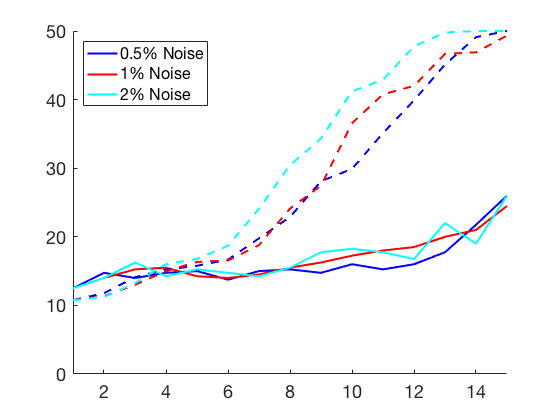
\includegraphics[width=0.7\linewidth]{Solver_stats}\\
  Average iterations per linear solve vs. outer iteration.  Solid
  lines for 4 largest values of $\lambda^{(\ell)}$, dashed lines for
  next 9 largest values.
\end{center}

\end{frame}

% - Begin Slide -----
\begin{frame}
  \frametitle{Trimming $\{\lambda^{(\ell)}\}$}

  Use na\"ive strategy for selecting smaller range of parameters at
  each outer iteration
  \begin{itemize}
  \item Aim to compute only around corner of L-curve
    \item Given optimal parameter from last outer iteration,
      $\lambda_{i-1}$, compute for 2 values of $\lambda^{(\ell)}$
      smaller than it, $\lambda_{i-1}$, and next 7 larger values
      \begin{itemize}
\item For first iteration, treat $\lambda_0 = \min_\ell
  \lambda^{(\ell)}$
  \item For small and large values of $\lambda_{i-1}$, adjust range to
    test 10 smallest/largest values of $\lambda^{(\ell)}$
      \end{itemize}
      
  \end{itemize}

  Gives small changes in performance of outer iteration
  \begin{itemize}
  \item For 2\% noise, $\lambda_{15} = 67.2$, relative error is 33.6\%
    \item For 1\% noise, $\lambda_{15} = 9.24$, relative error is 10.2\%
  \end{itemize}
  
  \end{frame}


% - Begin Slide -----
\begin{frame}
\frametitle{Range of $\{\lambda^{(\ell)}\}$}

For 1\% noise: \ \\[12pt]

\setlength\tabcolsep{5pt}
  \begin{tabular}{l|ccccc|ccccc|ccccc}
     & 1 & 2 & 3 & 4 & 5 & 6 & 7 & 8 & 9 & 10 & 11 & 12 & 13 & 14
    & 15 \\
    \hline
    small & 10  &  10   &  9 &    8  &   7&     6  &   5 &   5 &    3    & 2 &    1   &    &        &    &    \\
    med   &     &      &  1   &  2  &   3  &   4  &   5  &   5  &   7   &  8  &   9  &   9  &   8  &   7  &   6\\
    large &     &     &        &   &        &    &        &      &  
    &       &    &    1   &  2 &    3   &  4\\
    \end{tabular}

\ \\[6pt]
For 2\% noise: \ \\[12pt]

\setlength\tabcolsep{5pt}
  \begin{tabular}{l|ccccc|ccccc|ccccc}
     & 1 & 2 & 3 & 4 & 5 & 6 & 7 & 8 & 9 & 10 & 11 & 12 & 13 & 14
    & 15 \\
    \hline
    small & 10 &   10  &   8 &    5   &  3 &    2   &  1 &        &    &        &    &        &    &        &  \\
    med   &     &     &    2  &   5  &   7  &   8  &   9  &   9  &   8  &   7  &   6  &   6  &   6  &   6  &   6\\
    large &      &   &         &    &        &    &        &  1 &    2   &  3 &    4   &  4 &    4   &  4 &    4\\
  \end{tabular}

  \ \\[6pt]

  Solver statistics are similar to case where full range of
  $\{\lambda^{(\ell)}\}$ are tested.
\end{frame}


% - Begin Slide -----
\begin{frame}
\frametitle{Summary}
\vspace*{-9pt}
\begin{itemize}
\item X-ray CT inverse problem (Radon transform)
\item Nonlinear regularization approach leads to sequence of linear
  systems
\item Exhaustive search to optimize regularization parameter at each
  step
\item Solve rectangular linear systems using AMG technology
  \begin{itemize}
  \item Choice of relaxation scheme is key to performance
  \end{itemize}
\end{itemize}
\vspace*{-12pt}
\onslide*<2>{
\begin{center}
{\usebeamerfont{frametitle}\usebeamercolor[fg]{frametitle}Future Directions}
\end{center}
\vspace*{-12pt}
\begin{itemize}
\item Improve relaxation choice, particularly for moderate
  $\lambda^{(\ell)}$
\item Coarse-grid correction for small $\lambda^{(\ell)}$
\item Trim set of $\{\lambda^{(\ell)}\}$ considered for each outer
  iteration
\item Automated stopping criterion for outer iteration
  \item Other regularization terms, other models (deblurring)
\end{itemize}}%
\end{frame}

% - Begin Slide -----
\begin{frame}
  \frametitle{DD25}


  The 25th International Domain Decomposition Conference will be held
  in St.\ John's, NL, from July 23-27, 2018.
  \begin{itemize}
  \item Registration, submissions deadlines, to be announced
  \item Multigrid-focused minisymposium proposals welcome!
  \item Details (eventually) at \url{http://dd25.math.mun.ca/}
  \end{itemize}

\begin{center}
\onslide*<1>{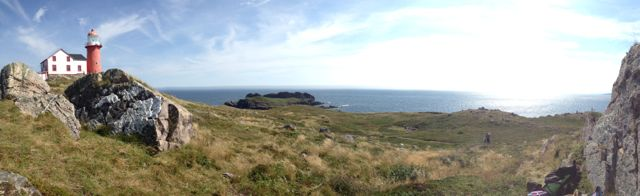
\includegraphics[width=0.95\linewidth]{new1_02.jpg}}%
\onslide*<2>{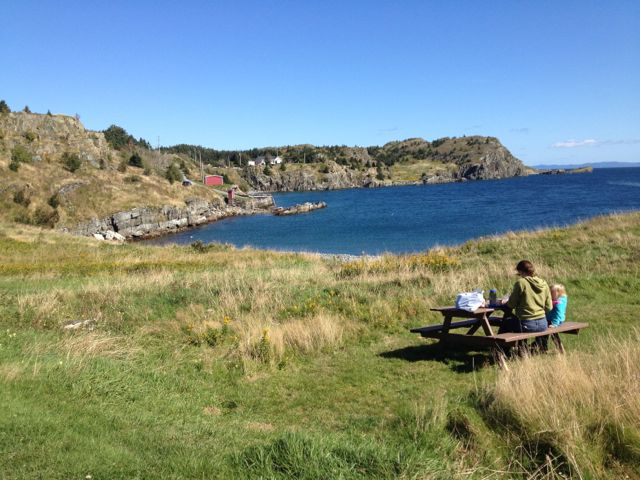
\includegraphics[width=0.5\linewidth]{new1_04.jpg}}%
\onslide*<3>{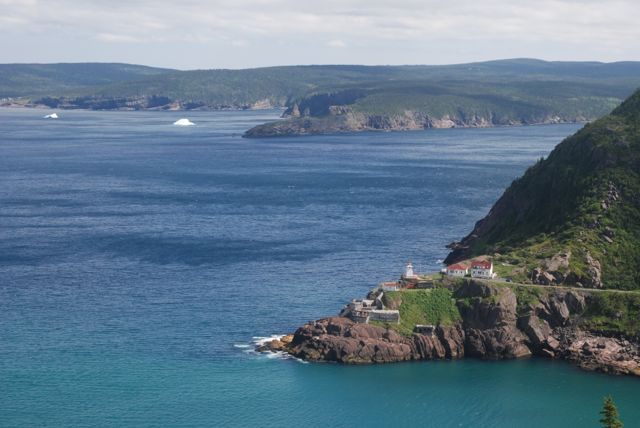
\includegraphics[width=0.58\linewidth]{new2_17.jpg}}%
\end{center}
  

\end{frame}



\end{document}

% - Begin Slide -----
\begin{frame}
\frametitle{}

\end{frame}

0.5% noise -> RelError 0.0065
1% noise -> RelError 0.0907
2% noise -> RelError 0.2978
